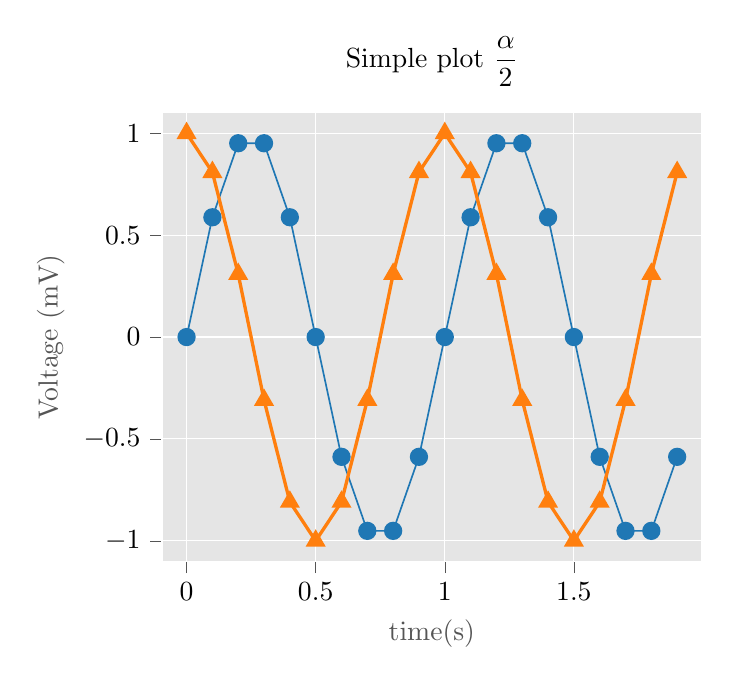
\begin{tikzpicture}

\definecolor{darkorange25512714}{RGB}{255,127,14}
\definecolor{dimgray85}{RGB}{85,85,85}
\definecolor{gainsboro229}{RGB}{229,229,229}
\definecolor{steelblue31119180}{RGB}{31,119,180}

\begin{axis}[
axis background/.style={fill=gainsboro229},
axis line style={white},
tick align=outside,
tick pos=left,
title={Simple plot \(\displaystyle \frac{\alpha}{2}\)},
x grid style={white},
xlabel=\textcolor{dimgray85}{time(s)},
xmajorgrids,
xmin=-0.095, xmax=1.995,
xtick style={color=dimgray85},
y grid style={white},
ylabel=\textcolor{dimgray85}{Voltage (mV)},
ymajorgrids,
ymin=-1.1, ymax=1.1,
ytick style={color=dimgray85}
]
\addplot [semithick, steelblue31119180, mark=*, mark size=3, mark options={solid}]
table {%
0 0
0.1 0.58778525
0.2 0.95105652
0.3 0.95105652
0.4 0.58778525
0.5 1.2246468e-16
0.6 -0.58778525
0.7 -0.95105652
0.8 -0.95105652
0.9 -0.58778525
1 -2.4492936e-16
1.1 0.58778525
1.2 0.95105652
1.3 0.95105652
1.4 0.58778525
1.5 3.6739404e-16
1.6 -0.58778525
1.7 -0.95105652
1.8 -0.95105652
1.9 -0.58778525
};
\addplot [very thick, darkorange25512714, mark=triangle*, mark size=3, mark options={solid}]
table {%
0 1
0.1 0.80901699
0.2 0.30901699
0.3 -0.30901699
0.4 -0.80901699
0.5 -1
0.6 -0.80901699
0.7 -0.30901699
0.8 0.30901699
0.9 0.80901699
1 1
1.1 0.80901699
1.2 0.30901699
1.3 -0.30901699
1.4 -0.80901699
1.5 -1
1.6 -0.80901699
1.7 -0.30901699
1.8 0.30901699
1.9 0.80901699
};
\end{axis}

\end{tikzpicture}
